\documentclass[12pt]{article}
\usepackage{graphicx}
\graphicspath{{imgs/}}
\usepackage{xeCJK}
\setCJKmainfont{Noto Serif CJK TC}
\usepackage[top=2cm, bottom=2cm, left=2cm, right=2cm, a4paper]{geometry}
\usepackage{setspace}
\setlength{\parskip}{2pt}
\usepackage{moresize}
\usepackage{placeins}
\usepackage{indentfirst}
\usepackage{amsmath}
\usepackage{caption, subcaption}

\begin{document}

\begin{center}
    \huge \textbf{EDA Final Project Report}
    
    \vspace{10pt}
    
    \large \textbf{110511010 楊育陞 110511067 葉哲伍}
\end{center}

\section{ICCAD 繳交截圖}

\section{Introduction}

\indent We take the \textbf{problem B} of the ICCAD contest as our final project. The problem is "Power and Timing Optimization Using Multibit Flip-Flop". Our method to solve this problem is mainly based on \textbf{clustering} and \textbf{gain-based greedy algorithm}. The clustering algorithm we use is inspired by the "Effective Mean Shift Algorithm" described in the paper "Graceful Register Clustering by Effective Mean Shift Algorithm for Power and Timing Balancing" \cite{jiang}.

\section{Method}

\subsection{Flowchart}

\begin{figure}[htbp]
    \centering
    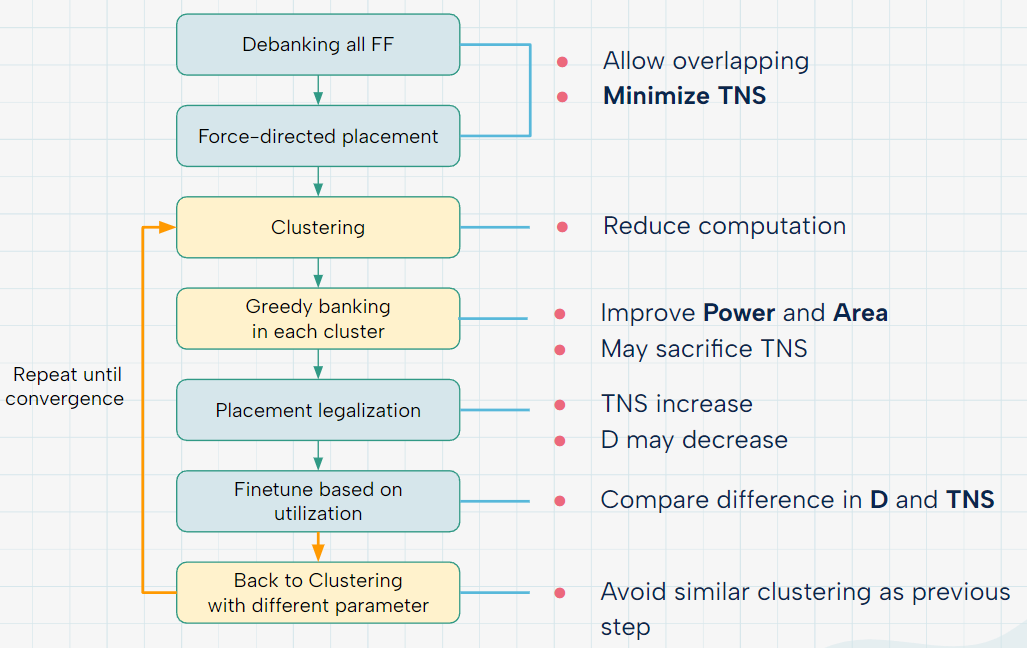
\includegraphics[width=0.9\textwidth]{flowchart2.png}
    \caption{Flowchart of our method}
    \label{fig:flowchart}
\end{figure}
\FloatBarrier

\subsection{Division of Labor}
\begin{itemize}
    \item 楊育陞: Debanking, Greedy banking, Finetuning based on utilzation
    \item 葉哲伍: Force-directed placement, Clustering, Placement legalization
\end{itemize}

\subsection{Detailed Explanation}

Our flow of the method is shown in Figure \ref{fig:flowchart}. We will explain each step in detail in the following subsections.

\subsubsection{Debanking all flip-flops}
In the initial given circuit, there are flip-flops of different bit-widths and different types. We first debank all flip-flops to single-bit flip-flops. The type of the single-bit flip-flop, called \textbf{base flip-flop} in our method, is chosen to be the single-bit flip-flop with the least cost calculated by the given cost function. The timing part of the cost is calculated by the q pin delay of the flip-flop in this step.

The debanking process is shown in Figure \ref{fig:debanking}. The debanked flip-flops are placed in the same position as the original flip-flops, and the connections are also kept the same. In this step, we allow the cells to overlap with each other.

\begin{figure}[htbp]
    \centering
    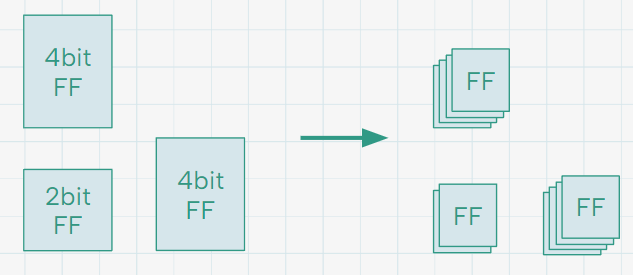
\includegraphics[width=0.7\textwidth]{debank.png}
    \caption{Debanking process}
    \label{fig:debanking}
\end{figure}

\subsubsection{Force-directed placement}
After debanking the flip-flops, we perform force-directed placement to determine the placement of the single-bit flip-flops. The force(weight) of each net is determined by the slack of the net. The first debanking step and this step are used to optimize the timing condition of the circuit.

In this problem, the cells are split into two types, combinational cells and flip-flops. The combinational cells are not allowed to move. So we should deal with two conditions when moving a flip-flop:

\begin{itemize}
    \item \textbf{All the connected cells of this flip-flop are combinational cells:} In this case, we can directly move the flip-flop to the timing optimal position.
    \item \textbf{There are flip-flops in the connected cells:} In this case, directly moving the flip-flop may not achieve the best timing condition since other connected flip-flops may move as well. So we should consider the movement of the connected flip-flops and the movement of the flip-flop itself. We use a iterative greedy method to solve this problem: We move one flip-flop at a time and fix the position of the other flip-flops. We repeat this process until the positions of all flip-flops are fixed or the distances converge.
\end{itemize}

For this step, we introduce a \textbf{"lock" mechanism} to achieve high efficiency. The lock mechanism is used to lock the position of the flip-flops that have been placed in the optimal position or the distances for several iterations have converged. The locked flip-flops will not be moved in the following iterations. Since the condition 1 discussed above will lock the flip-flop in the first iteration, \textbf{there is no need to consider which condition the flip-flop belongs to}, highly improving the efficiency of the algorithm.

\subsubsection{Clustering}

Our clustering algorithm is inspired by the "Effective Mean Shift Algorithm" described in the paper "Graceful Register Clustering by Effective Mean Shift Algorithm for Power and Timing Balancing" \cite{jiang}. However, we have made some modifications to adapt it to our specific needs. \textbf{Instead of directly applying the clustering algorithm for power and timing balancing, we use it to create clusters of flip-flops for our next step, which is greedy banking.} This allows us to optimize the time complexity of the greedy banking process by performing it on smaller clusters rather than on all flip-flops at once. Additionally, we believe that the greedy banking process should only consider nearby flip-flops within each cluster, which further improves its efficiency.

In this step, there are two part of parameters to be tuned:
\begin{itemize}
    \item \textbf{Bandwidth:} The bandwidth of the clustering algorithm. This parameter determines the size of the cluster. A larger bandwidth will result in fewer clusters, while a smaller bandwidth will result in more clusters. Fewer clusters may lead to a better banking result, but it also increases the time complexity of the greedy banking process.
    \item \textbf{Effective Negihbors:} The number of effective neighbors of a flip-flop. This parameter determines the number of flip-flops that are considered as neighbors of a flip-flop when calculating the mean shift. This parameter mainly affects the runtime of the clustering algorithm.
\end{itemize}

\subsubsection{Greedy banking in each cluster}

After clustering the flip-flops, we perform the greedy banking algorithm in each cluster. The greedy banking algorithm is as follows:

\begin{enumerate}
    \item Calculate the gain of all pairs of flip-flops in the cluster. The gain of a pair of flip-flops is defined as \textbf{the reduction of the cost function if the two flip-flops are banked together and placed in the optimal position using the force-directed placement algorithm}. The cost function is provided in the problem as follows, here the penalty term $D$ is ignored in this step:
    $$
    \sum_{\forall i \in FF}(\alpha \cdot TNS(i) + \beta \cdot Power(i) + \gamma \cdot Area(i)) + \lambda \cdot D
    $$
    \item Choose the pair of flip-flops with the highest gain and bank them together.
    \item Repeat step 1 and 2 until no pair of flip-flops has a positive gain.
\end{enumerate}


After the greedy banking process, the positions of the flip-flops are updated, and the connections are also updated accordingly. This may lead to non-optimal timing conditions in this state. So we need to \textbf{perform the force-directed placement algorithm again} to optimize the timing condition.

\subsubsection{Placement legalization}

The above steps would lead to illegal placements as they allow the flip-flops to overlap with each other. So we need to perform placement legalization to avoid the overlap of flip-flops. Our placement legalization algorithm is as follows:

\begin{enumerate}
    \item 
\end{enumerate}

\subsubsection{Finetuning based on utilization}

\subsubsection{Back to clustering with different parameters}

\subsection{Parallelization}

When designing our method, we carefully considered the potential for parallelization. We will explain the potential for parallelization in each step:

\begin{itemize}
    \item \textbf{Debanking:} This step can be parallelized by debanking different flip-flops in parallel since there is no overlap between different flip-flops in the initial circuit.
    \item \textbf{Force-directed placement:} This step can be parallelized by moving different flip-flops in parallel. \textbf{To avoid conflicts, we allow the flip-flops to overlap with each other in this step.}
    \item \textbf{Clustering:} This step can be parallelized by mean shifting different flip-flops in parallel as in the original paper.
    \item \textbf{Greedy banking:} This step can be parallelized by applying the greedy banking algorithm to different clusters in parallel.
\end{itemize}

Since the runtime of our program in this contest is limited, we want to make the best use of the parallelization to improve the efficiency of our method. But the implementation of parallelization is relatively complex, so we consider to implement it in the clustering and greedy banking steps first, which are the most time-consuming steps in our method.


\section{Result}

\section{Conclusion}

\begin{thebibliography}{9}
    \bibitem{jiang} 
    Ya-Chu Chang, Tung-Wei Lin, Iris Hui-Ru Jiang, and GiJoon Nam. "Graceful Register Clustering by Effective Mean Shift Algorithm for Power and Timing Balancing." \textit{Proceedings of the 2019 International Symposium on Physical Design (ISPD '19)}, 2019.
\end{thebibliography}

\end{document}
